\section{Introduction}
When working with images, it is often usual to use a smaller representation of the original image.
This can usually achieved by scaling down the image or cropping it. This write-up will show why resizing and cropping are not the best methods to achieve it and introduce better solutions like \textit{bidirectional similarity} \cite{bisi} and \textit{inverse texture synthesis} \cite{its}. 

\begin{figure}[h]
\centering
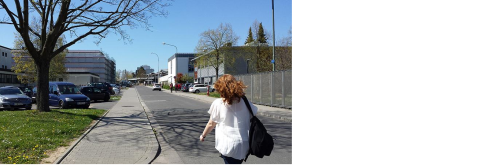
\includegraphics[scale=0.9]{img/ShrinkingCropping}
\caption[Image shrinking]{The original upper image shows parts of the University of Mainz with view towards
the mensa at the end of street and a person in front. (a) was normally shrunk and (b) was shrunk by using content aware scaling of Adobe Photoshop\footnotemark. (c) is a result of cropping, focusing on the mensa.}
\label{fig:Image shrinking}
\end{figure}
\footnotetext{Further reading at Adobe Helpcenter: https://helpx.adobe.com/photoshop/using/content-aware-scaling.html}


\subsection{Shrinking images}
Shrinking images is probably the fastest way to get the desired smaller representation of the image. A big advantage of shrinking images is that the layout of the image remains as it was before. On the other hand the smaller image loses quality of the resolution and the change of aspect ratio causes distortion. Figure \ref{fig:Image shrinking} (a) shows a normal downscaled image. As expected, the person on it does not look natural anymore because of the distortion.\\
Figure 1 (b) shows another method of image shrinking which uses the paradigma of importance-based scaling where unimportant parts get more downscaled than important parts. So, compared with (a), the person and the tree look way more natural, but the sidewalk disappears because of different scalings.



\subsection{Cropping images}
Cropping images is another fast way to obtain a smaller representation. Figure 1 (c) shows a cropped image. Unlike (a) and (b) the quality of resolution in (c) stays equal, but as clearest disadvantage every information outside the cropped area gets lost. \\
Cropping also comes in importance-based versions which work well on images with concentrated important regions, so that the lost parts only consist of unimportant information.\\
The disadvantages of both methods, shrinking and cropping, are too significant for satisfying results. The following two sections will introduce two better methods.
